\documentclass[
    10pt % font size
    16:9, % 1920x1080
]{beamer}
% \usetheme{default}
% \usetheme{Boadilla}
 \usetheme{Madrid}
% \usetheme{Montpellier}
% \usetheme{Warsaw}
% \usetheme{Copenhagen}
% \usetheme{Goettingen}
% \usetheme{Hannover}
% \usetheme{Berkeley}
 
% \usecolortheme{crane}
 % \beamertemplatesolidbackgroundcolor{craneorange!25}
 
 % Define custom colors
\definecolor{customGreen}{RGB}{0,128,0} % A medium green
\definecolor{customDarkGreen}{RGB}{0,100,0} % A darker green

% Apply the custom colors
\usecolortheme{default} % Start with the default color theme to apply custom colors on top
\setbeamercolor{structure}{fg=customGreen}
\setbeamercolor{background canvas}{bg=white} % Set main background to white
\setbeamercolor{title}{bg=customDarkGreen,fg=white} % Title slide background
\setbeamercolor{frametitle}{bg=customGreen,fg=white} % Frame titles

% Custom footline with an image on the bottom right
\addtobeamertemplate{footline}{}{%
  \hfill%
  \raisebox{5mm}[0pt][10pt]{%
    
\includegraphics[height=1cm]{kyu_univ_logo.png}%
  }\hspace*{5mm}
}

\title{StoryWeaverGPT}
\subtitle{Dataset, Tokenizer and Embedding}

\author{Group1}

\begin{document}

\frame{\titlepage} % # 1
\section[Outline]{}
\frame{\tableofcontents}

\section{Introduction}
 
 
\frame % # 2
{
  \frametitle{Dataset and Tokenizer}
 
  \begin{itemize}
    \item Dataset: Reddit WritingPrompts Dataset
    \item Tokenizer: BPE Tokenizer
  \end{itemize}
  
\vfill   
}

\section{Dataset}
 
 \frame % # 2
{
  \frametitle{Dataset: WritingPrompts Dataset}
  % image
  \begin{figure}
    \centering
    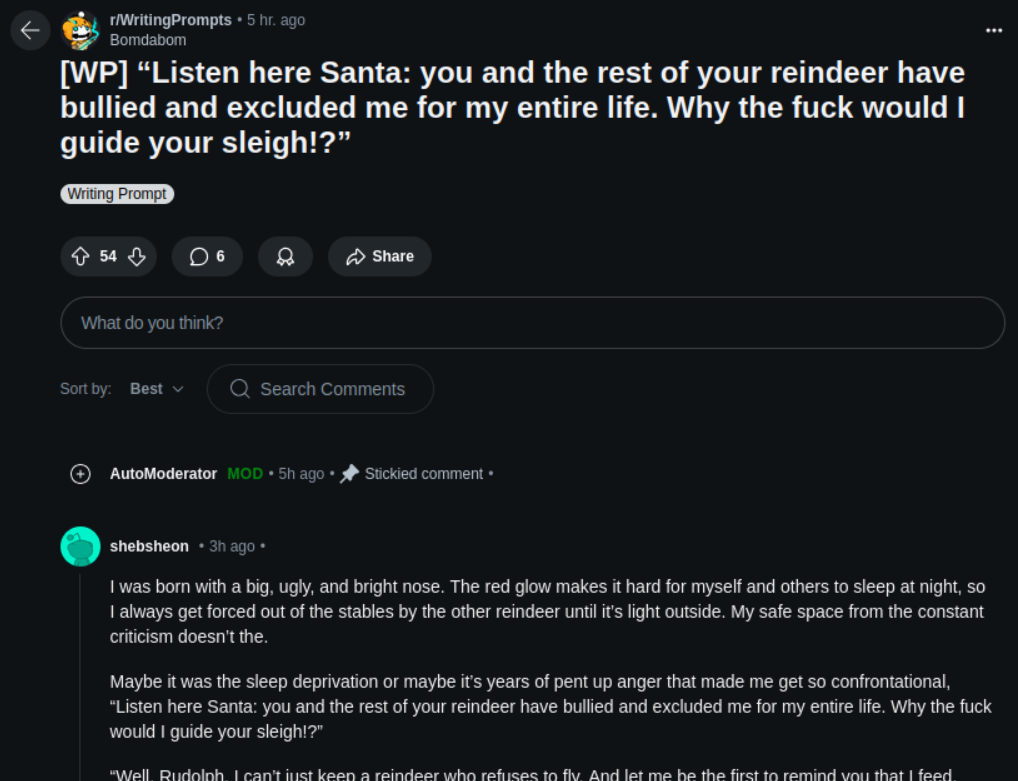
\includegraphics[width=0.7\textwidth]{dataset.png}
    \caption{WritingPrompts Dataset}
  \end{figure}
}


\section{Tokenizer}
 
\frame
{
  \frametitle{Tokenizer: BPE Tokenizer}
  
  \begin{itemize}
      \item Iteratively merge the most frequent pairs of tokens to build a subword vocabulary.
  \end{itemize}

  \begin{table}[]
      \centering
      \begin{tabular}{|c|c|c|}
          \hline
          Iteration & Tokens & Most Frequent Pair \\ \hline
          Initial   & h e l l o & l l \\ \hline
          1         & h e ll o  & e ll \\ \hline
          2         & h ell o   & h ell \\ \hline
          3         & hell o    & None \\ \hline
      \end{tabular}
      \caption{Example of BPE Tokenization for "hello"}
  \end{table}
  
  \begin{itemize}
      \item Key Idea: The sequence evolves by merging pairs to minimize the overall vocabulary size while retaining meaning.
  \end{itemize}
}

\frame{
  \frametitle{Tokenizer: BPE Tokenizer}
  \begin{itemize}
      \item BPE Tokenizer performs better when trained on same dataset as dataset the main model is being trained on
      \item Our tokenizers are trained on the WritingPrompts dataset, with 8192 merges.
      \item With multiprocessing training took 28 hours.
  \end{itemize}
}


 \frame
{
  \frametitle{Tokenizer Code}
  \begin{figure}
    \centering
    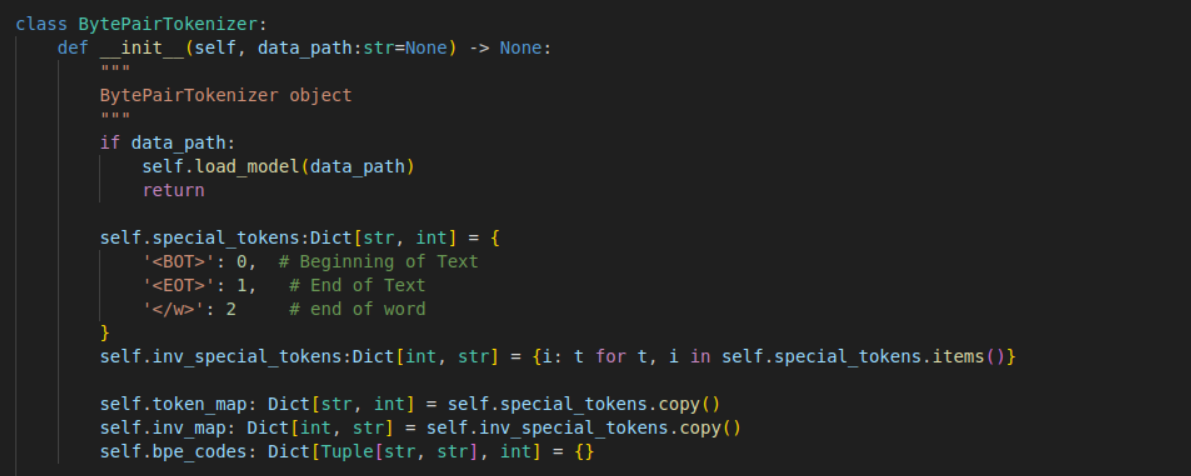
\includegraphics[width=0.8\textwidth]{tokenizer_init.png}
    \caption{Initializing Tokenizer}
  \end{figure}

}

\frame
{
  \frametitle{Tokenizer Code}
  \begin{figure}
    \centering
    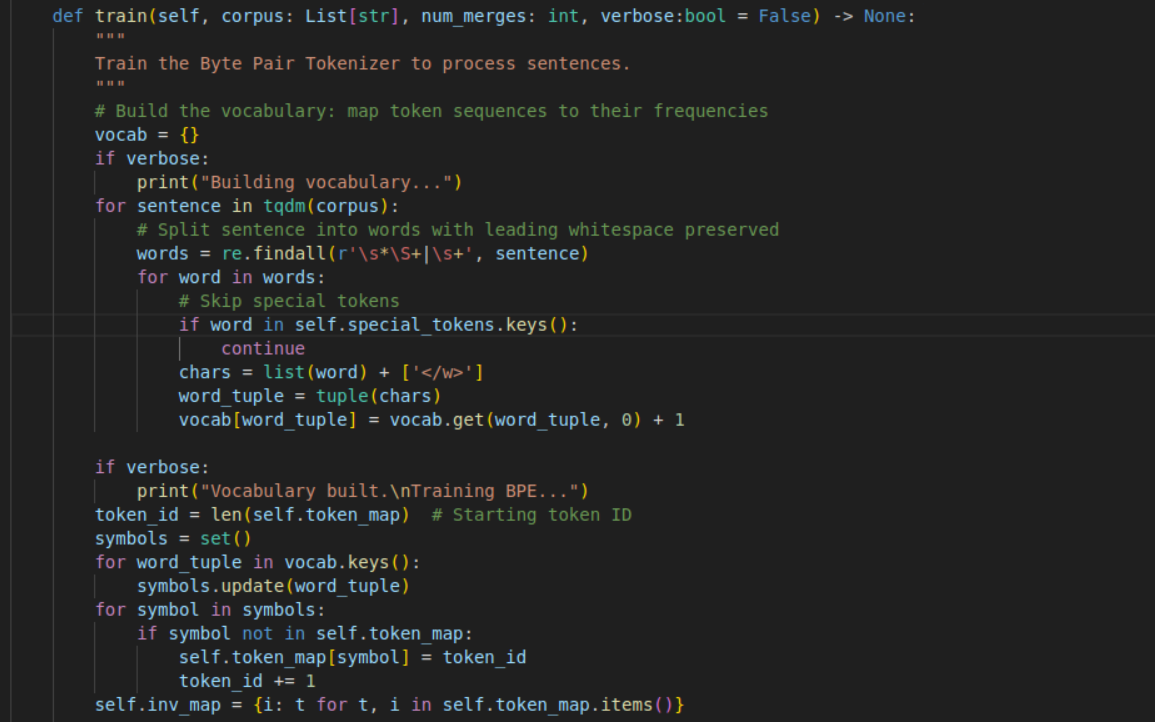
\includegraphics[width=0.8\textwidth]{train_tokenizer.png}
    \caption{Counting Frequency}
  \end{figure}
}

\frame
{
  \frametitle{Tokenizer Code}
  \begin{figure}
    \centering
    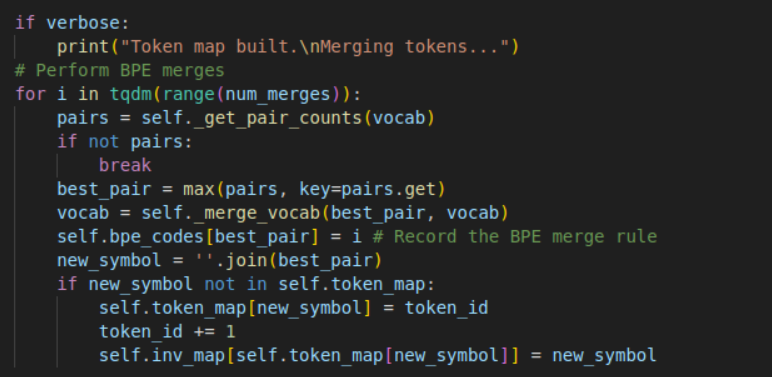
\includegraphics[width=0.8\textwidth]{train_tokenizer2.png}
    \caption{Performing Merges}
  \end{figure}
}

\frame
{
  \frametitle{Tokenizer Code}
  \begin{figure}
    \centering
    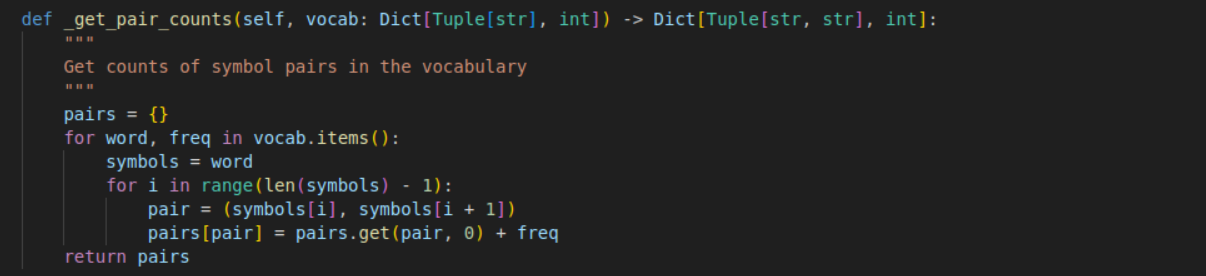
\includegraphics[width=0.8\textwidth]{get_pair_count.png}
    \caption{get\_pair\_count}
  \end{figure}
}
\frame
{
  \frametitle{Tokenizer Code}
  \begin{figure}
    \centering
    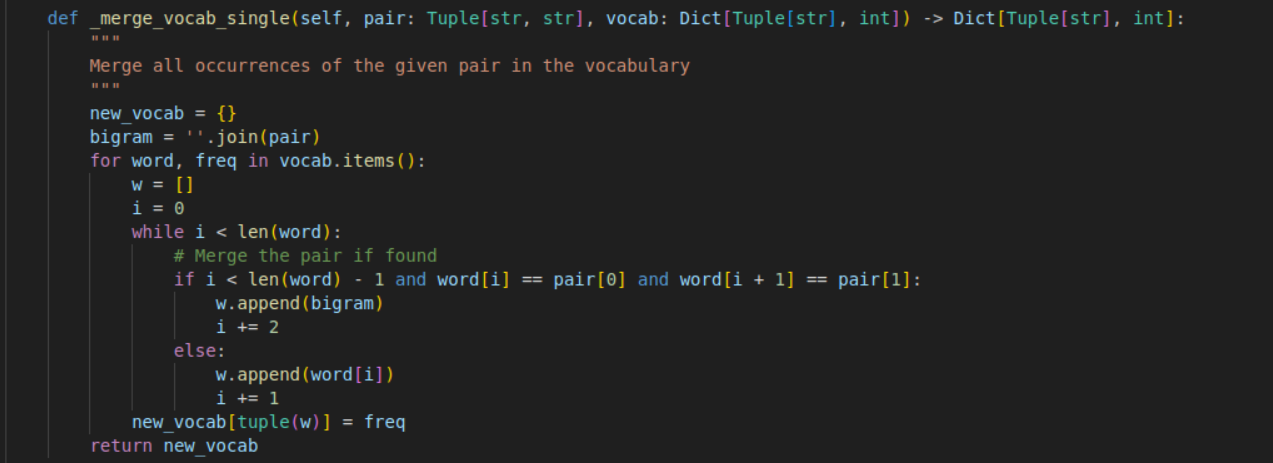
\includegraphics[width=0.8\textwidth]{merge_vocab_single.png}
    \caption{merge\_pair}
  \end{figure}
}
\frame
{
  \frametitle{Tokenizer Code}
  \begin{figure}
    \centering
    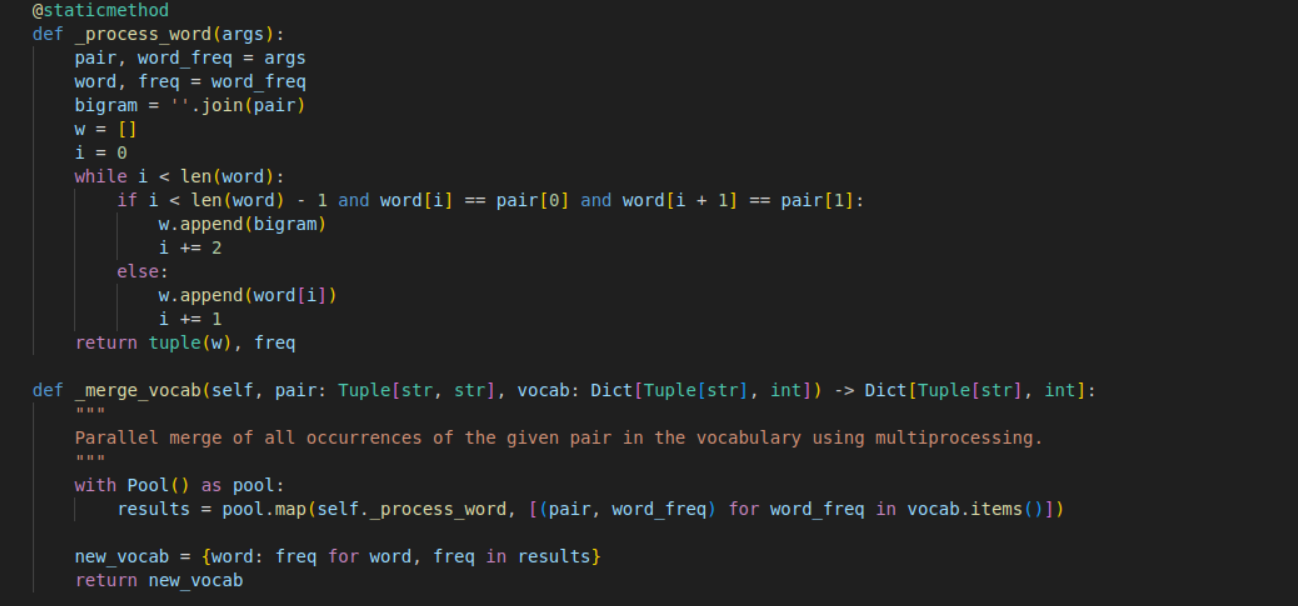
\includegraphics[width=0.8\textwidth]{merge_pair.png}
    \caption{merge\_pair}
  \end{figure}
}

\frame
{
  \frametitle{Tokenizer Code}
  \begin{figure}
    \centering
    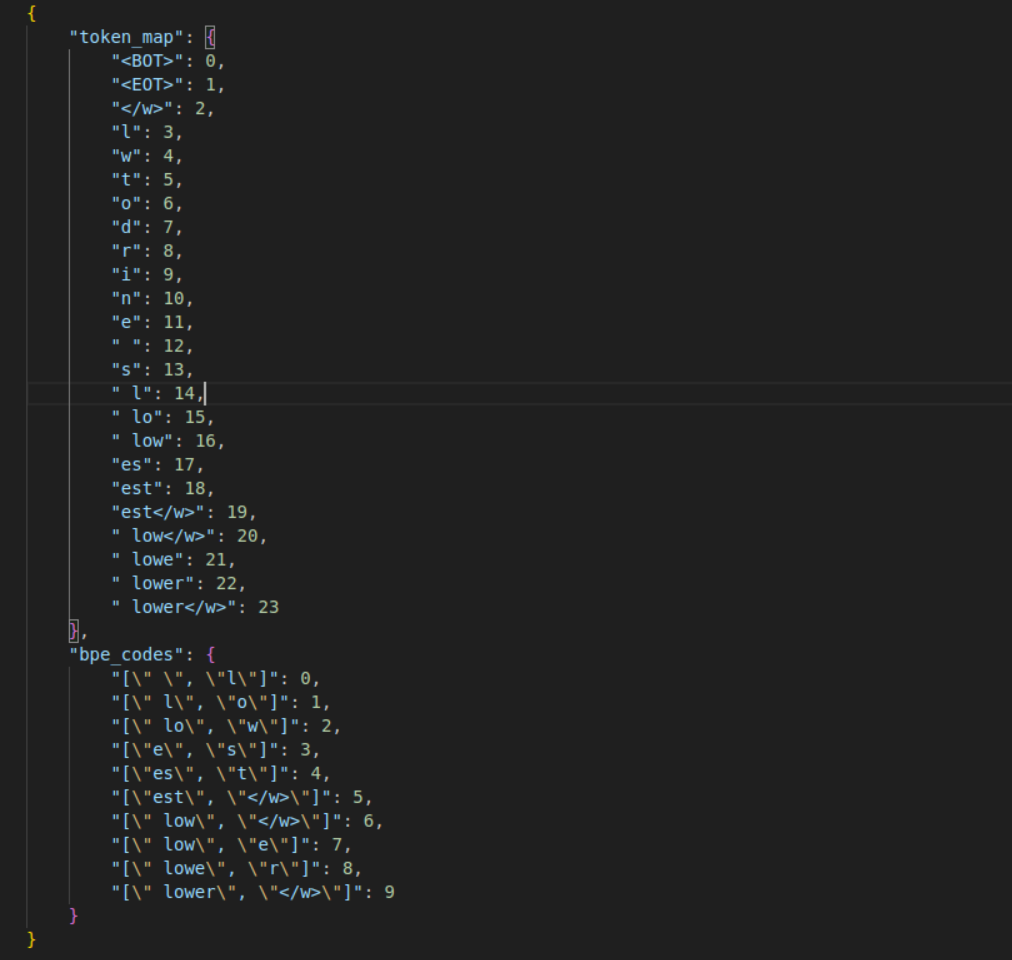
\includegraphics[width=0.6\textwidth]{tokenized_model.png}
    \caption{Sample model}
  \end{figure}
}

\section{Embedding}

\frame
{
  \frametitle{Embedding}
  \begin{itemize}
      \item Embedding is a linear map from a one-hot encoded vector to  a dense vector.
      \item $E: \mathbb{R}^{V} \rightarrow \mathbb{R}^{d}$
      \item Where V is vocab dimension, and d is the embedding dimension.
      \item This is first linear map/layer applied to tokenized input, and is learned with the model.
  \end{itemize}
  \begin{figure}
    \centering
    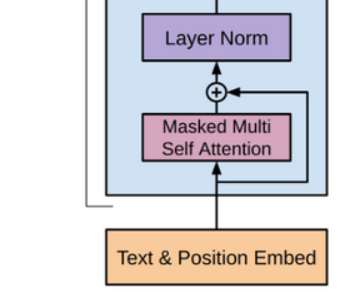
\includegraphics[width=0.3\textwidth]{model.png}
  \end{figure}
}

\frame
{
  \frametitle{Embedding}
  \begin{figure}
    \centering
    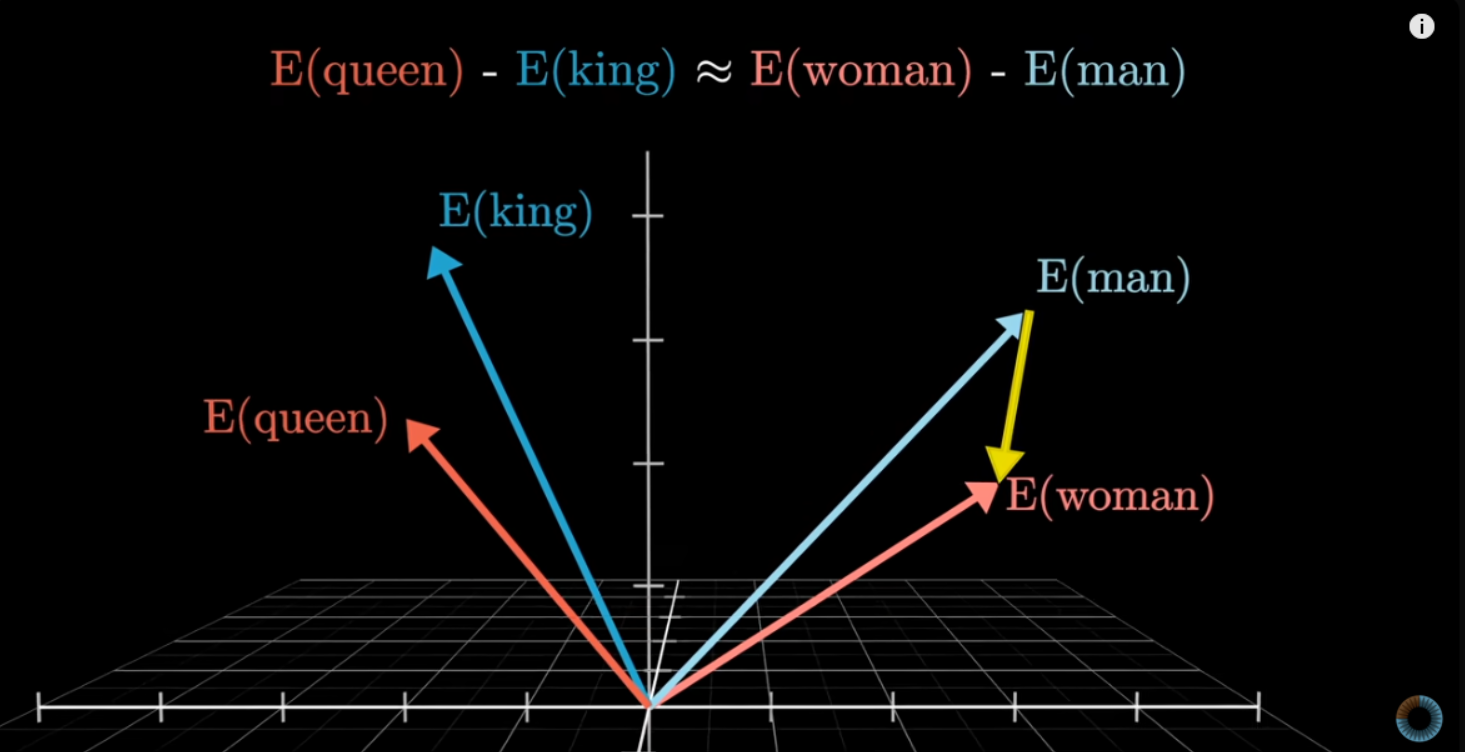
\includegraphics[width=0.7\textwidth]{3blue1brown.png}
    \caption{Demonstration of Embedding space}
  \end{figure}
}

\frame
{
  \frametitle{Embedding}
  \begin{figure}
    \centering
    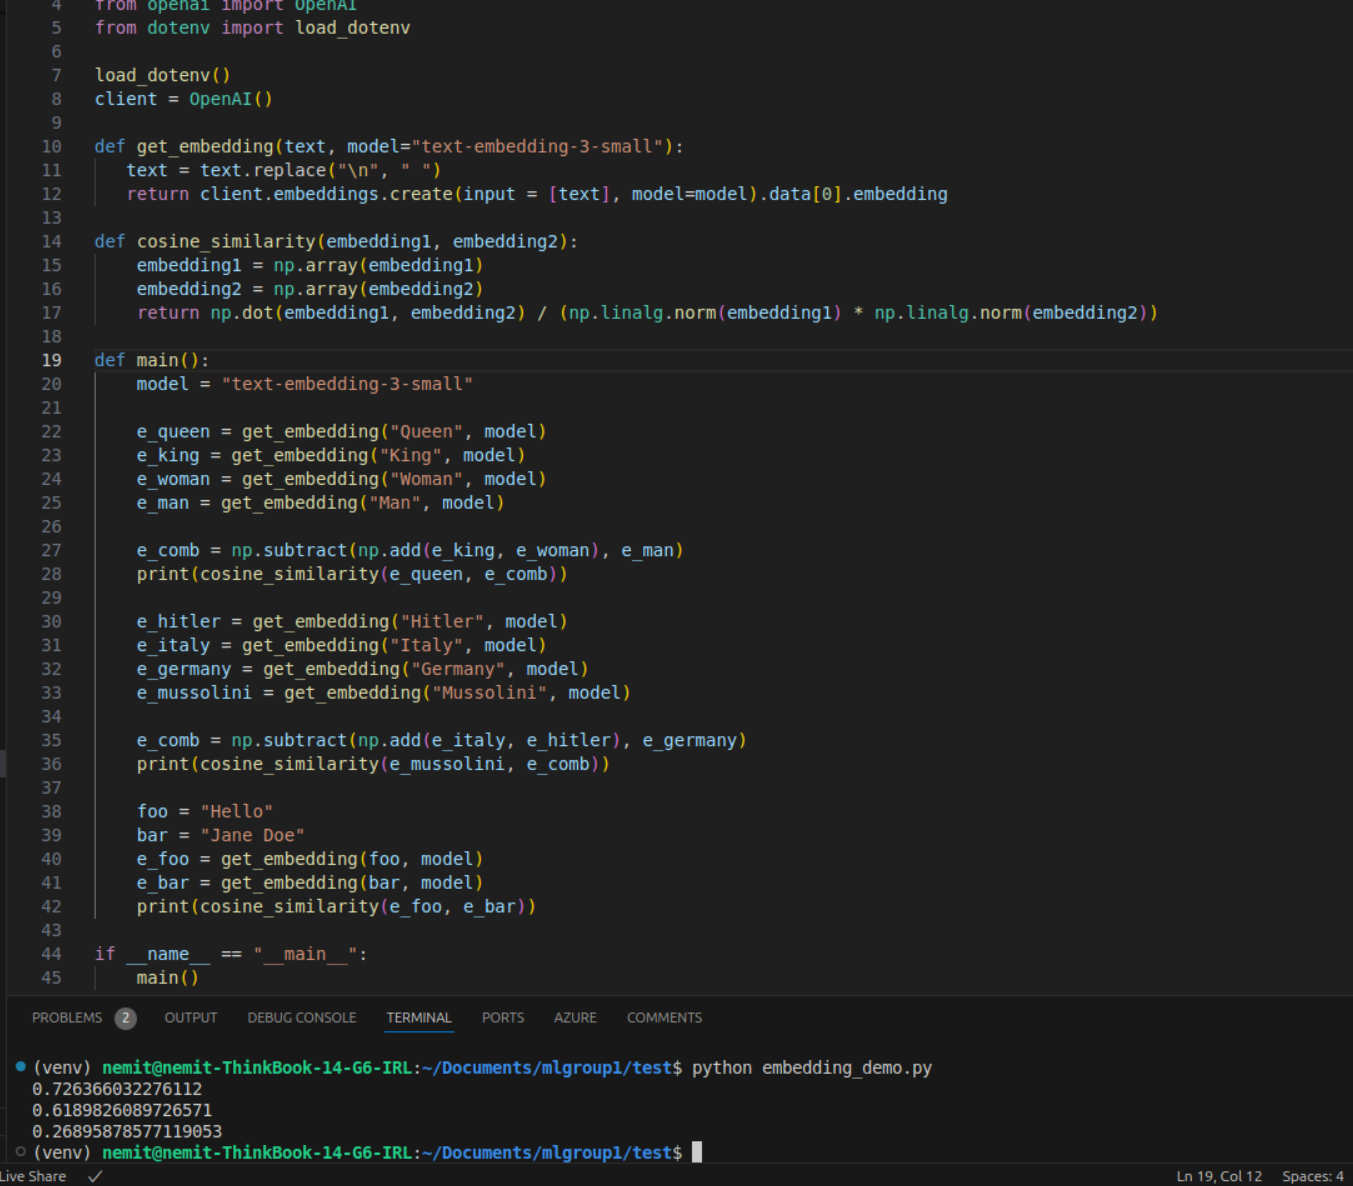
\includegraphics[width=0.7\textwidth]{similarity.png}
  \end{figure}
}

\frame
{
  \frametitle{Embedding}
  \begin{itemize}
      \item Outside NLP/NLG model, embeddings are used for similarity, clustering, and visualization.
      \item RAG, Retrival Augmented generation, uses embeddings to retrive relevant information.
  \end{itemize}
}

\frame
{
  \frametitle{Positional Encoding}
  \begin{itemize}
      \item Positional encoding is added to embeddings to give the model information about the position of the token.
      \item Positional encoding is a sine and cosine function of the position.
      \item $$P[i, j] = \begin{cases}
        \sin\left(\frac{i}{10000^{2j/d}}\right) & \text{if j is even} \\
        \cos\left(\frac{i}{10000^{2j/d}}\right) & \text{if j is odd}
      \end{cases}$$
  \end{itemize}
}

\frame
{
  \frametitle{Embedding and Positional Encoding Code}
  \begin{figure}
    \centering
    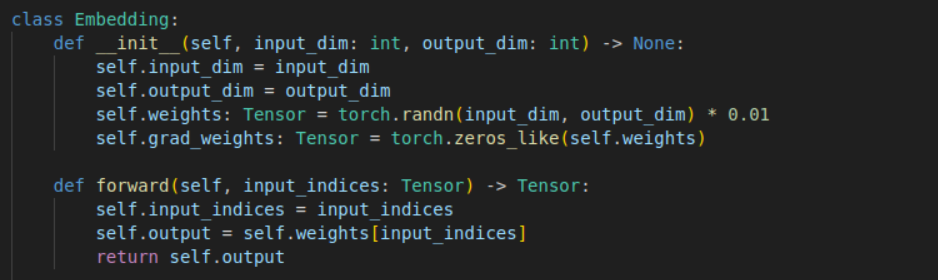
\includegraphics[width=0.8\textwidth]{embedding_code.png}
    \caption{Embedding Class}
  \end{figure}
  \begin{figure}
    \centering
    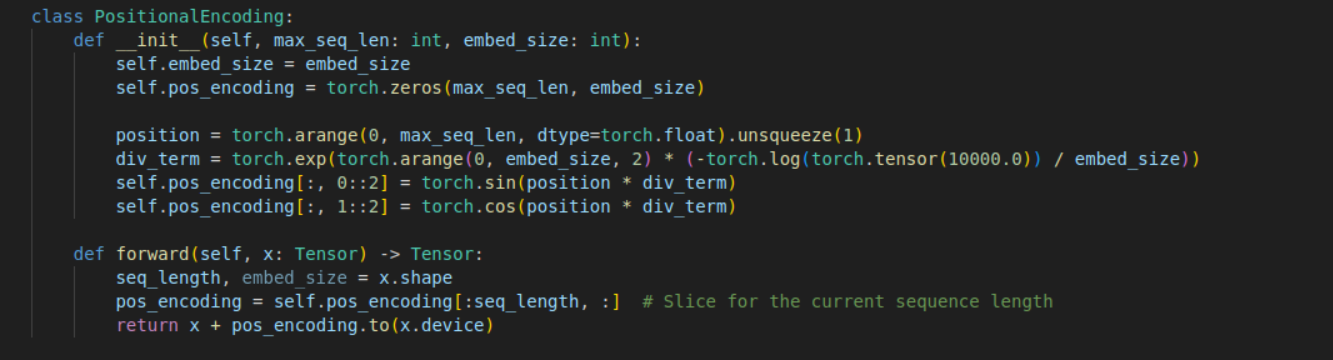
\includegraphics[width=0.8\textwidth]{pos_code.png}
    \caption{Positional Encoding}
  \end{figure}
}

\frame
{
  \frametitle{Next Steps}
  \begin{itemize}
    \item Attention and Feedforward block for a Transformer block.
    \item Output projection layer and Calculating loss.
  \end{itemize}
}
\end{document}
       
 